\documentclass[a4paper, 12pt]{article}

\usepackage{geometry}
\usepackage{textcomp}					% "true" символы типа copyright

\usepackage{cmap}						% Улучшенный поиск русских слов в полученном pdf-файле
\usepackage[T2A]{fontenc}				% Поддержка русских букв
\usepackage[utf8]{inputenc}				% Кодировка utf8
\usepackage[english, russian]{babel}	% Языки: русский, английский
\usepackage[unicode]{hyperref}			% Русский язык для оглавления pdf
\usepackage{bookmark}					% Оглавление в pdf
\usepackage{soulutf8}					% Для разрядки

\usepackage{amssymb,amsmath,amsthm}
\usepackage{graphicx} 					% Подключаем пакет работы с графикой
\usepackage[ruled]{algorithm}
\usepackage[noend]{algpseudocode}

\usepackage{color}

\usepackage{titlesec}					% Форматирование заголовков
%\usepackage{abstract}					% Форматрирование абстракта	

\geometry{a4paper,top=2cm,bottom=2cm,left=2.5cm,right=1cm}	% Геомтерия страницы
\graphicspath{{../../images/}} 			% Пути к изображениям

% Настройка теоремоподобных окружений
\theoremstyle{plain}
\newtheorem{Theorem}{Теорема}
\newtheorem{Lemma}[Theorem]{Лемма}
\newtheorem{Pred}{Утверждение}
\newtheorem{Corollary}{Следствие}
\newtheorem{Def}{Определение}
\newenvironment{Proof}%
	{\par\noindent{\bf Доказательство.}}%
	{\hfill$\scriptstyle\blacksquare$}

\floatname{algorithm}{}
\newcommand{\algrule}[1][.2pt]{\par\vskip.2\baselineskip\hrule height #1\par\vskip.2\baselineskip}
\algrenewcommand\algorithmicrequire{\textbf{Вход:}}
\algrenewcommand\algorithmicensure{\textbf{Выход:}}
\algrenewcommand\algorithmicforall{\textbf{для всех}}
\algrenewcommand\algorithmicwhile{\textbf{пока}}
\algrenewcommand\algorithmicif{\textbf{если}}
\algrenewcommand\algorithmicthen{\textbf{то}}
\algrenewcommand\algorithmicelse{\textbf{иначе}}
\algrenewcommand\algorithmicreturn{\textbf{вернуть}}
\algrenewcommand\algorithmicfunction{\textbf{процедура}}
\algrenewcommand\algorithmicdo{}
\renewcommand{\algorithmiccomment}[1]{{\quad\sl // #1}}

\renewcommand\labelenumi{\theenumi )}	% Нумерованный перечень со скобками
\AtBeginDocument{\renewcommand{\abstractname}{\vspace{-2\baselineskip}}}    		% clear the title
%\renewcommand{\absnamepos}{empty} % originally center

\makeatletter
	\bibliographystyle{gost2008p}
	\renewcommand{\@biblabel}[1]{#1.}	% Заменяем библиографию с квадратных скобок на точку:
\makeatother

\titleformat{\section}[runin]{\normalfont\bfseries}{\thesection.}{1pt}{}[.]
\titleformat{\subsection}[runin]{\normalfont}{\thesubsection.}{1pt}{\so}[.]
%\titleformat{command}[shape]{format}			   {label}		 {sep}{before}[after]

\DeclareMathOperator*{\argmax}{arg\,max}
\DeclareMathOperator*{\argmin}{arg\,min}

\title{\hbox{\normalsize\textit{УДК 004.81}}\hbox{}\textbf{\Large\MakeUppercase{Управление поведением как функция сознания. II. Самосознание и синтез плана}}\footnote{Работа выполнена при поддержке РНФ (грант \No\ 14-11-00692).}}
\author{\textbf{\textcopyright~2015~г. Г.\,С.~Осипов, А.\,И.~Панов, Н.\,В.~Чудова}\\\normalsize\textit{Москва, Институт системного анализа РАН}}
\date{}

\begin{document}
	\vspace*{-5\baselineskip}			% Убираем лишние пробелы перед заголовком статьи
	{\let\newpage\relax\maketitle}
	
	\begin{abstract}
		\noindent Рассматривается семантический уровень описания функций, которые в психологии принято относить к функциям сознания и самосознания. Исследуется механизм работы компонент знака, введённых в первой части статьи.На основе описания знака на семантическом уровне исследуется сходимость основного итерационного процесса образования знака "--- связывания образной компоненты знака и его значения. Введение алгоритмов работы компонент знака позволяет построить алгоритм процесса синтеза плана поведения, а также построить новую архитектуру интеллектуальных агентов, обладающих, в частности, способностями к распределению ролей в коалициях.
	\end{abstract}	
	
	\section*{Введение}
	Как было подробно изложено в первой части статьи \cite{PanovA2014a}, в качестве базовых психологических теорий, в которых даётся не только качественное описание свойств когнитивных функций, но и приводятся структурные описания лежащих в их основе психических образований, в предложенном подходе  использованы культурно-исторический подход Выготского"--~Лурии \cite{Luria1970,Vygotsky2005}, теория деятельности Леонтьева \cite{Leontiev1975} и модель психики Артемьевой \cite{Artemyeva1980}. Согласно приведённым теориям высшие сознательные когнитивные функции осуществляются в рамках так называемой мотивированной предметной деятельности, когда объекты и процессы внешней  среды опосредованы для субъекта специальными образованиями, называемыми знаками. Благодаря наличию четырёх компонент: образа, значения, личностного смысла и имени "--- знак участвует в реализации тех или иных когнитивных функций. 
	
	Четырёхкомпонентная структура элемента индивидуального знания, которая как было сказано выше, в психологии называется знаком, подтверждается и теми работами нейрофизиологов, в которых предпринимается попытка построить общую теорию работы мозга человека. Так, в теории повторного входа Эделмена \cite{Edelmen1981} и Иваницкого \cite{Ivanitsky1996,Ivanitsky2010} утверждается, что образование осознанного ощущения или фиксация входного потока информации происходит только в том случае, когда активированное сенсорным входом возбуждение через ассоциативные зоны коры от гиппокампа, а затем от гипоталамуса накладывается на сенсорный след в проекционной коре. Такой <<круг ощущений>> (рис. \ref{fig:ivan_cyrcle}), проходящий за характерное время в 150-300 мс, последовательно активирует три компоненты индивидуального знания: образную (проекционная и сенсорная зоны коры), компоненту значения (гиппокамп) и личностного смысла (гипоталамус). Регистрация сигнала в лобных долях (после возврата его в зоны первичной проекции), по видимому, связано с именованием всех трёх уже активированных компонент.
	
	\begin{figure}[h]
		\centering
		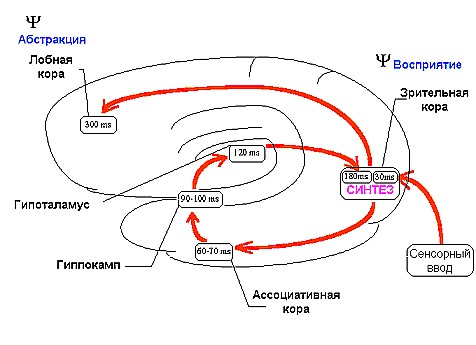
\includegraphics[width=0.7\linewidth]{ivanitsky_cyrcle}
		\caption{<<Круг ощущений>> по Иваницкому \cite{Ivanitsky1996}.}
		\label{fig:ivan_cyrcle}
	\end{figure}
	
	Кроме того, по современным нейрофизиологическим представлениям строение коры головного мозга практически однородно во всём своём объёме, о чём свидетельствует наличие колонок некоротекса \cite{Mountcastle1998,Rockland2010}. При этом связи между достаточно малыми зонами коры (так называемый коннектом \cite{Zador2012}), явно указывают на иерархичность ее строения и на присутствие как восходящих, так и обратных, нисходящих связей. Отсюда следует, что основные компоненты элемента индивидуального знания должны обладать иерархическим однородным строением с восходящими потоками информации и нисходящей обратной связью. Кроме того, образная компонента должна иметь такую функцию распознавания, которая кроме категоризации статических объектов и динамических процессов использует обратную связь для предсказания сигнала в следующий момент времени.
	
	\section{Семантические уровень}
	В качестве модели базовой составляющей основных компонент знака будем использовать специальный распознающий автомат ($R$-автомат), основными функциями которого являются следующие функции:
	\begin{itemize}
		\item хранение информации $\mathcal Z$ о множестве некоторых сходных явлений (предметов и процессов внешнего мира), которые будем называть множеством выходных признаков $F^*$ этого автомата,
		\item распознавание выходных признаков по информации о множестве входных признаков $F$ с помощью множества функций распознавания $\hat F$.
	\end{itemize}
	
	Действие функции распознавания заключается в сопоставлении каждому признаку $f_k^*$ из множества $F^*$ действительного значения $x_k^*$ по входному вектору $\bar x$. Значение $x_k^*$ определяет уровень доверия тому, насколько успешно удалось построить признак из составляющих его низкоуровневых признаков, взвешенные значения присутствия которых определяются вектором $\bar x$.
	
	В соответствии с данными нейрофизиологии будем считать, что множество $R$-автоматов $\mathcal R$ организовано в иерархическую схему в виде связного ориентированного ярусного графа. Выходная информация от распознающего автомата $R_i^j\in\mathcal R$ направляется на нижний уровень иерархии, на вход поступает, соответственно, информация с верхнего уровня. Нижний индекс распознающего автомата является сквозным по множеству $\mathcal R$, а верхний обозначает номер яруса, которому принадлежит автомат.
	
	Опишем множества входных $A$, выходных сигналов $B$ и множество состояний $Q$ распознающего автомата  $R_i^j=<A_i^j,Q_i^j,B_i^j,\varphi_i^j, \eta_i^j>$ или просто $R=<A,Q,B,\varphi, \eta>$.
	$R$-автомат принимает на вход пару векторов $(\bar x,\hat x^{j+1})$, где первый вектор является вектором весов входных признаков размерности $q$, а второй "--- входным управляющим вектором с верхнего уровня иерархии размерности $l$, который принимает ненулевое значение только в фиксированные для данного автомата моменты времени $0,h,2h,\dots$. Таким образом, множество входных сигналов $A$ является декартовым произведением пространства взвешенных векторов входных признаков $X$ и пространства управляющих векторов с верхнего уровня иерархии $\hat X^{j+1}$: $A=X\times \hat X^{j+1}$. 
	
	На выходе $R$-автомат выдаёт пару $(\bar x^*,\hat x^j)$, где $\bar x^*$ "--- это вектор весов выходных признаков размерности $l$, а $\hat x^j$ "--- выходной управляющий вектор на нижний уровень иерархии размерности $q$, который с учётом других автоматов уровня $j$ является входным управляющим вектором для некоторых автоматов уровня $j-1$. Из этого следует, что за единицу времени для автоматов уровня $j$ проходит $h^{j-1}$ единиц времени для автоматов уровня $j-1$. Таким образом, выходное множество $B$ является декартовым произведением пространства взвешенных векторов выходных признаков $X^*$ и пространства управляющих векторов для нижнего уровня иерархии $\hat X^j$: $A=X^*\times \hat X^j$.
	
	Будем считать множество состояний конечным, в связи с чем каждой функции распознавания $\hat f_k$ из множества $\hat F$ будем ставить в соответствие набор матриц предсказания $Z_k=\{Z_1^k,…,Z_m^k\}$ размерности $q\times h$, где $h$ "--- характерное время распознающего автомата. Столбец $\bar{z}_u^r=(z_{u1}^k,…,z_{uq}^k)$ матрицы $Z_r^k$ интерпретируется как вектор предсказания присутствия входных признаков из множества $F$ в момент времени $\tau+u$, где $\tau = 0,h,2h,\dots$. При этом $z_{uv}^k\in\{0,1\}$, т.~е. вектор $\bar{z}_u^r$ является булевым вектором. Сама матрица $Z_r^k$ задаёт, таким образом, последовательность событий, наличие которых свидетельствует о~присутствии распознаваемого функцией $\hat f_k$ признака. Иными словами, множество всех матриц предсказания распознающего автомата $\mathcal Z$ хранит в себе информацию о выходных признаках. Множество состояний будем определять как совокупность всех подмножеств множества всех матриц предсказания: $Q=2^{\mathcal Z}$.
	
	Таким образом, распознающий автомат $R$ является бесконечным автоматом Мили с переменной структурой и конечной памятью: $R_i^j=<X\times\hat X^{j+1}, 2^{\mathcal Z}, X^*\times\hat X^j,\varphi_i^j,\eta>$ (рис. \ref{fig:rb_io}). Алгоритм $\mathcal A_{th}$ вычисления функции переходов $\varphi$ и выходной функции $\eta$ по начальному моменту времени $\tau$, управляющему воздействию $\hat x^{j+1}(\tau)$ и входному воздействию $\omega_i^j$ представлен ниже. В алгоритме используется стандартная функция $W$ нормировки весовых значений:
	\begin{equation}
	W(\bar x)=\left(\frac{x_1}{\max\limits_i x_i},\dots,\frac{x_n}{\max\limits_i x_i}\right),
	\end{equation} 
	где $\bar x=(x_1,\dots,x_n)$ "--- вектор с ненормированными компонентами.
	
	\begin{algorithm}
		\caption{Алгоритм $\mathfrak{A}_{th}$}\label{alg:automato}
		\begin{algorithmic}[1]
					\Require $\tau_s, \hat{x}_i^{j+1}(\tau_s), \omega_i^j$.
		\Ensure $\varphi_{i\Delta t}^j, \vec\eta_{i\Delta t}^j$.

		\State $\hat{F}^*=\varnothing,Z^*=\varnothing,t=0$; \Comment{активные функции распознавнаия и матрицы предсказания}
		\State $c_1\in(0,1), c_2\in(0,1)$; \Comment{пороговые константы}

		\Statex \Comment{определение начального состояния}
				
		\ForAll{компонент $\hat{x}_{ik}^{j+1}$ вектора $\hat{x}_i^{j+1}(\tau_s)=(\hat{x}_{i1}^{j+1},\hat{x}_{i2}^{j+1},\dots,\hat{x}_{il}^{j+1})$} \label{alst:init_start}
			\If{$\hat{x}_{ik}^{j+1}{\ge}c_1$} \label{alst:select_f}
				\State $\hat{F}^*:=\hat{F}^*\cup\{\hat{f}_k\}$;
			\EndIf
		\EndFor
		
		\State $\bar x_i^j:=\omega_i^j(\tau_s)$;
		
		\ForAll{функций распознавания $\hat{f}_k\in\hat{F}^*$}
			\ForAll{$Z_r^k\in Z_k$, соответствующих функции распознавания $\hat{f}_k$,}
				\If{$\frac{\|\bar{z}_1^r-\bar{x}_i^j\|}{\|\bar{z}_1^r\|+\|\bar{x}_i^j\|}<c_2$} \label{alst:select_z}
					\State $Z^*:=Z^*\cup\{Z_r^k\}$;
				\EndIf
			\EndFor
		\EndFor
		
		\State $\varphi_i^j(\bar x_i^j,\hat{x}_i^{j+1}(\tau_s)) := Z^*$; \Comment{значение функции переходов в начальный момент времени}\label{alst:init_state}
		\State $\bar N:=(|\{Z_r^1|Z_r^1\in Z^*\}|,\dots,|\{Z_r^{l_i^j}|Z_r^{l_i^j}\in Z^*\}|)$; \label{alst:init_calc_out2}
		\State $\eta(Z^*)=\bar{x}_i^{*j}:=W(\bar N)$; \Comment{значение функции выходов в начальный момент времени} \label{alst:init_calc_out3}
		\State $\hat x_i^j=W(\sum_{\hat f_k\in\hat F^*}\hat x_{ik}^{j+1}\sum_{Z_r^k\in Z^*}\bar z_2^r)$;\label{alst:init_control}
		\label{alst:init_end}
				\Statex \Comment{основной цикл}
	
	\State $t=1$;
	\While{$t\leqslant{h_i^j}-1$} \label{alst:cycle_start}
		\State $\bar{x}_i^j:=\omega(\tau_s+t)$;
	
		\ForAll{матриц предсказания $Z_r^k$ из множества $Z^*$}
			\If{$\frac{\|\bar{z}_{t+1}^r-\bar{x}_i^j\|}{\|\bar{z}_{t+1}^r\|+\|\bar{x}_i^j\|}\geqslant{c_2}$} \label{alst:update_z}
				\State $Z^*:=Z^*\setminus\{Z_r^k\}$;
			\EndIf
		\EndFor
	
		\State $\varphi_i^j(\bar x_i^j,\hat{x}_i^{j+1}(\tau_s)) := Z^*$; \Comment{значение функции переходов в момент времени $t$}
		\State $\bar N=(|\{Z_r^1|Z_r^1\in Z^*\}|,\dots,|\{Z_r^{l_i^j}|Z_r^{l_i^j}\in Z^*\}|)$; \label{alst:calc_out1}
		\State $\eta(Z^*)=\bar{x}_i^{*j}:=W(\bar N)$;\Comment{значение функции выходов в момент времени $t$} \label{alst:calc_out3}
	
		\State $t=t+1$;
		\If{$t\leqslant{h}_i^j-2$}
			\State $\hat{x}_i^j:=W(\sum_{\hat f_k\in\hat F^*}\hat x_{ik}^{j+1}\sum_{Z_r^k\in Z^*}\bar z_t^r)$; \label{alst:calc_state1}
		\EndIf
	\EndWhile \label{alst:cycle_end}
		\end{algorithmic}
	\end{algorithm}
	
	\begin{figure}[H]
		\centering
		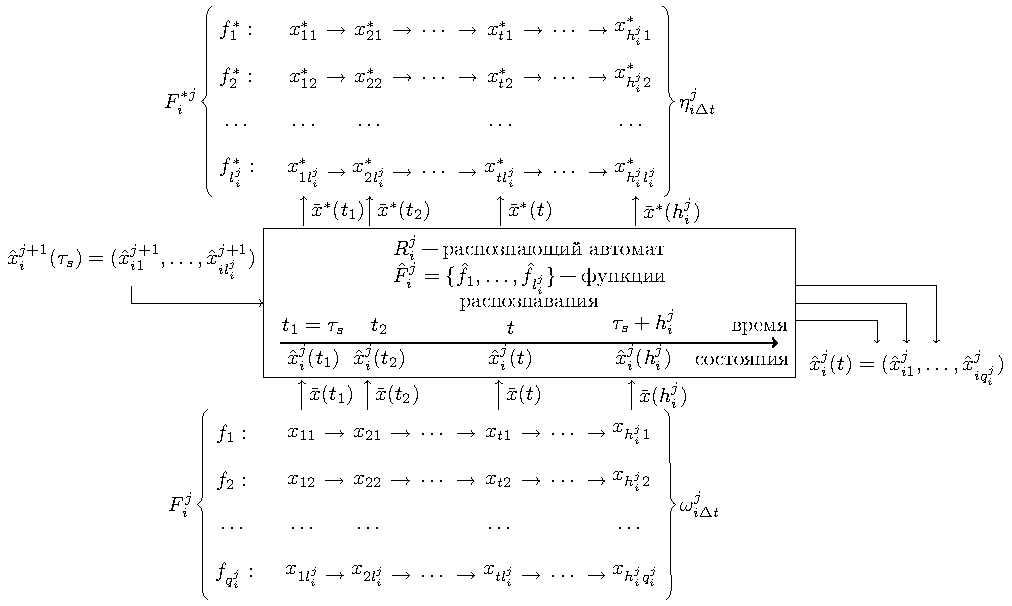
\includegraphics[width=1.0\linewidth]{rb_io}
		\caption{Входные и выходные сигналы распознающего автомата.}
		\label{fig:rb_io}
	\end{figure}
	
	\subsection{Определение компонент знака}
		Для определения компонент знака через описанный в предыдущем разделе $R$-автомат необходимо ввести ряд вспомогательных понятий. 
		
		Введём семейство бинарных отношений $\{\sqsubset,\sqsubset^1,\sqsubset^2,\dots\}$, определённых на декартовом произведении $\{f_k\}\times \{f_k\}$. Будем считать, что <<признак $f_1$ является составляющим признака $f_2$>> или <<признак $f_2$ измеряется по признаку $f_1$>>, $(f_1,f_2 )\in\sqsubset$ или $f_1\sqsubset f_2$, в том случае, если $f_1\dashv R_1^j, f_2\dashv R_2^{j+1}$, $R_2^{j+1}$ "--- родительский блок по отношению к $R_1^j$ и в множестве матриц предсказания $\mathcal Z_2$ признака $f_2$ существует как минимум одна матрица $Z_r^2$, содержащая некоторый столбец $\bar z_u^r$ с элементом $z_{uv}^r\not=0$, где $v$ "--- индекс признака $f_1$ во входном векторе для распознающего блока $R_2^{j+1}$.
		
		Пара признаков $(f_1,f_2)\in\sqsubset^t$ или $f_1\sqsubset^t f_2$, где $t\in\{1,2,\dots\}$, в~том случае, если $f_1\dashv R_1^j, f_2\dashv R_2^{j+1}$, $R_2^{j+1}$ "--- родительский блок по отношению к $R_1^j$ и в множестве матриц предсказания $\mathcal Z_2$ признака $f_2$ существует как минимум одна матрица $Z_r^2$, содержащая $t$–ый столбец $\bar z_t^r$ с~элементом $z_{tv}^r\not=0$, где $v$ "--- индекс признака $f_1$ во~входном векторе для распознающего блока $R_2^{j+1}$.
		
		Каждый элемент векторов"--~столбцов соотносится с~признаком из~входного множества признаков распознающего блока, что означает задание типа для каждого элемента вектора"--~столбца. Будем обозначать тип $k$-го элемента вектора-столбца распознающего блока $R_i^j$ как $f_i^j(k)\in F_i^j$, $k\in(1,q_i^j)$. 
		
		Введём два выделенных из множества $\{f_k\}$ признака: $f_c$ "--- <<условие>> и $f_e$ "--- <<эффект>>, распознаваемые одним распознающим блоком $R_0^1$: $F_0^{*1}=\{f_c,f_e\}$. Те признаки, которые распознаются распознающими блоками, выступающими родительскими по отношению к блоку $R_0^1$, будем называть процедурными признаками, остальные "--- объектными признаками.
		
		Для любого процедурного признака выполняются следующие естественные условия:
		\begin{itemize}
			\item условие всегда предшествует эффекту,
			\item условие всегда влечёт за собой эффект и
			\item все условия всегда отделены от своих эффектов.
		\end{itemize}
		
		Иными словами, если $f_1$ "--- процедурный признак, то если в столбце $\bar z_u^r$ матрицы предсказания $Z_r^1$ элемент $z_{uv}^r$, соответствующий признаку $f_c$, не равен $0$, то в этом столбце соответствующий признаку $f_e$ элемент вектора "--- нулевой, в столбце $z_{u+t}^r, t>0$ наоборот "--- элемент $z_{u+t,v}^r$, соответствующий признаку $f_c$, равен $0$, а соответствующий признаку $f_e$ элемент "--- не нулевой. Те столбцы матрицы предсказания $Z$, в которых соответствующий признаку $f_e$ элемент вектора не нулевой, будем называть \textit{столбцами эффектов}, а те столбцы матрицы предсказания $Z$, в которых не равен нулю элемент вектора, соответствующий признаку $f_c$ "--- \textit{столбцами условий}. 
		
		Пополним семейство отношений $\{\sqsubset,\sqsubset^1,\sqsubset^2,\dots\}$ двумя отношениями: $\sqsubset^c$ и $\sqsubset^e$, принадлежность к~которым пары признаков $(f_1,f_2)$ свидетельствует о~том, что признак $f_1$ присутствует соответственно в~столбце условий и эффектов как минимум в~одной матрице предсказания процедурного признака $f_2$.
		
		\begin{Def}
			Если $f_1$ "--- признак, то подмножество $\tilde p(f_1)$ множества $\{f_k\}$ таких признаков, что $\forall f_i\in\tilde p(f_1) f_i\sqsubset f_1$, будем называть перцептом признака $f_1$.
		\end{Def}
		
		На множестве всех перцептов $\tilde P$ введём величину $\rho_p(\tilde p(f_1),\tilde p(f_2))$, вычисляемую по~следующему правилу:
		\begin{itemize}
			\item если $f_1$ и $f_2$ распознаются разными распознающими блоками, т.~е. $f_1\dashv R_1^j, f_2\dashv R_2^i$, то $\rho_p(\tilde p(f_1),\tilde p(f_2))=\infty$,
			\item если $f_1$ и $f_2$ распознаются одним и тем~же распознающим блоком $R_1^j$ со~множеством входных признаков $F_1^j$ мощности $q$ и характерным временем $h$, то
			\begin{equation}
				\rho_p(\tilde p(f_1),\tilde p(f_2))=\min\limits_{\substack{Z_r^1\in Z_1\\Z_s^2\in Z_2}}\frac{1}{q\cdot h}\sum\limits_{u=1}^h\|\bar z_u^r-\bar z_u^s\|.
			\end{equation} 
		\end{itemize}
		
		\begin{Pred}
			Величина $\rho_p$ является метрикой на множестве перцептов $\tilde P$.
		\end{Pred}
		
		\begin{Def}
			Если $f_1$ "--- признак, $f_2$ "--- процедурный признак, $f_1\sqsubset^c f_2$, то будем называть $f_2$ функциональным значением признака $f_1$. Множество всех функциональных значений признака $f_1$ будем обозначать $\tilde m(f_1)$.
		\end{Def}
		
		На множестве всех функциональных значений $\tilde M$ введём величину $\rho_m(\tilde m(f_1),\tilde m(f_2))$, вычисляемую по следующему правилу:
		\begin{equation}
			\rho_m(\tilde m_1(f_1),\tilde m_2(f_2 ))=\min\limits_{\substack{f_i\in\tilde m(f_1 )\\f_j\in\tilde m(f_2 )}}\rho_p(\tilde p(f_i ),\tilde p(f_j )).
		\end{equation}
		
		\begin{Pred}
			Величина $\rho_m$ является метрикой на множестве функциональных значений $\tilde M$.
		\end{Pred}
		
	\subsection{Семантический уровень обобщения} Определение ролевой структуры для алгоритма планирования.
	
	\noindent\colorbox{yellow}{
		\parbox{\dimexpr\linewidth-2\fboxsep}{Здесь я бы предложил дать определение типам обобщения на семантическом уровне.}
	}
	
	\section{Связывание образа и значения}
		Для формальной записи итерационного процесса связывания образа и значения в алгоритме образования знака из первой части статьи рассмотрим подробнее строение матрицы предсказания процедурного признака. Матрицу предсказания $Z_r^p$ процедурного признака $f_p$ всегда можно представить в следующем виде:
		\begin{equation}
		Z_r^p=(\bar z_1^{r,c},\dots,\bar z_{j_1}^{r,c},\bar z_{j_{1+1}}^{r,e},\dots,\bar z_{i_1}^{r,e},\dots,\dots,\bar z_{i_{k-1}+1}^{r,c},\dots,\bar z_{j_k}^{r,c},\bar z_{j_k+1}^{r,e},\dots,\bar z_{i_k}^{r,e}),
		\end{equation}
		где $\bar z_j^{r,c}$ "--- столбцы причин, $\bar z_i^{r,e}$ "--- столбцы следствий. 
		
		Величину $k$ будем называть актностью процедурного признака. В~дальнейшем будем рассматривать простые матрицы предсказаний $k$-актного процедурного признака:
		\begin{equation}
		Z_r^p=(\bar z_1^{r,c},\bar z_2^{r,e},\dots,\dots,\bar z_{2\cdot k-1}^{r,c},\bar z_{2\cdot k}^{r,e}).
		\end{equation}
		Краткая форма $k$-актного процедурного признака $f_p$ имеет матрицу предсказания, в которой оставлены только первый столбец условий и последний столбец эффектов.
		
		Любой одноактный процедурный признак $f_p$, распознаваемый блоком $R_i^j$, можно представить в виде правила $r_p=(F_C(f_p),F_A(f_p),F_D(f_p))$, в котором:
		\begin{itemize}
			\item $F_C (f_p )\subseteq F_i^j$ "--- множество признаков "--- условий правила: $\forall f\in F_C(f_p)$ $f\sqsubset^c f_p$;
			\item $F_A(f_p)\subseteq F_i^j$ "--- множество добавляемых правилом признаков: $\forall f\in F_A(f_p)$ $f\sqsubset^e f_p,f\notin F_C$;
			\item $F_D(f_p)\subseteq F_i^j$ "--- множество удаляемых правилом признаков: $\forall f\in F_D(f_p)$ $f\notin F_A,f\in F_C$.
		\end{itemize}
		
		Очевидно, выполняются следующие соотношения: $F_A(f_p)\cap F_D(f_p)=\varnothing, F_A(f_p)\cap F_C(f_p)=\varnothing, F_D(f_p)\subseteq F_C(f_p)$.
		
		\begin{Def}
			Процедурный признак $f_p^1$ c матрицей предсказания $Z=(\bar z_1^c,\bar z_2^e)$ выполняется на векторе $z$ длины $q$, если $z\cdot \bar z_1^c=\bar z_1^c$.
		\end{Def}
		Будем говорить, что процедурный признак $f_p^1$ выполним в~условиях процедурного признака $f_p^2$, если 
		\begin{itemize}
			\item оба признака распознаются одним и тем~же распознающим блоком $R_i^j$ и признак  $f_p^1$ выполняется на~столбце условий матрицы предсказания признака $f_p^2$,
			\item $f_p^1\dashv R_1^{j_1}, f_p^2\dashv R_2^{j_2}$, множества $F_C(f_p^1 )$ и $F_C(f_p^2)$ состоят из~одних и тех~же признаков, образуемый вектор $\tilde z$ (той же мощности, что и множество $F_1^{j_1}$) элементы которого, соответствующие признакам из $F_C(f_p^2)$ принимаются равными $1$,  остальные "--- $0$, и признак $f_p^1$ выполним на~векторе $\tilde z$. 
		\end{itemize}
		
		\begin{Def}
			Будем говорить, что два процедурных признака $f_p^1$ и $f_p^2$ конфликтуют, если выполнено как минимум одно из~следующих условий:
			\begin{itemize}
				\item $F_D(f_p^1)\cap F_A(f_p^2)\not=\varnothing$,
				\item $F_D(f_p^2)\cap F_A(f_p^1)\not=\varnothing$,
				\item $F_D(f_p^1)\cap F_C(f_p^2)\not=\varnothing$,
				\item $F_D(f_p^2)\cap F_C(f_p^1)\not=\varnothing$.
			\end{itemize}
		\end{Def}
		
		\begin{Def}
			Результатом операции сохраняющего приведения вектор"--~столбца $\bar z_1$ к~множеству входных признаков $F_{i_2}^{j_2}$ будем называть такой вектор $\bar z_3$ длины $q_{i_2}^{j_2}$, элемент которого $z_{3k}=1$, если $f_{i_1}^{j_1}(k)=f_{i_2}^{j_2}(k)$ и $z_{1k}=1$, иначе $z_{3k}=0$, и обозначать $(\bar z_1\rightarrow F_{i_2}^{j_2})=\bar z_3$.
		\end{Def}
		
		\begin{Def}
			Результатом операции сужающего приведения вектор"--~столбца $\bar z_1$ к~некоторому столбцу $\bar z_2$ распознающего блока $R_{i_2}^{j_2}$ будем называть такой вектор $\bar z_3$ длины $q_{i_2}^{j_2}$, элемент которого $z_{3k}=1$, если $f_{i_1}^{j_1}(k)=f_{i_2}^{j_2}(k)$, $z_{2k}=1$ и $z_{1k}=1$, иначе $z_{3k}=0$, и обозначать $(\bar z_1\Rightarrow \bar z_2)=\bar z_3$.
		\end{Def}
		
		Будем считать, что у субъекта имеется опыт наблюдения, который выражается в виде отношения $\Psi_p^m$: $\tilde p\Psi_p^m \tilde m$, или $\Psi_p^m(\tilde p)=\tilde m$, в том случае, если $\tilde p\in\tilde P$ является перцептом некоторого признака $f$, а $\tilde m\in\tilde M$ "--- функциональным значением того же признака $f$.
		
		Ниже представлен алгоритм доопределения функции $\Psi_p^m$, который и отражает собой суть итерационного процесса во время образования знака согласно алгоритму из первой части статьи. Доопределение проводится на~новую пару $(\tilde p,\tilde m)$, где функциональное значение $\tilde m$ строится в сравнении с эталоном $\tilde m^0$, а перцепт $\tilde p$ формируется на основе подмножества составляющих признаков $\hat F$. Доопределение функции $\Psi_p^m$ означает формирование нового признака $f^*$, т.~е. его первой матрицы предсказания $Z^*$ в~рамках распознающего блока $R^*$.
				
	\begin{algorithm}
		\caption{Алгоритм $\mathfrak{A}_{pm}$}\label{alg:pm}
		\begin{algorithmic}[1]
			\Require $\tilde m^0=\{f_p\}, \Psi_p^m, \hat F\subseteq \{f_k\}$;
			\algrule
			
			\State $\tilde p^{*(0)} := \varnothing$;
			\State $Z^{*(0)} := \varnothing$;
			\State $t := 0$;
			\ForAll{$f^{(t)}\in \hat F$}
			\If{$\exists \tilde m^{(t)}\in \tilde M$ такое, что $(\tilde p(f^{(t)}),\tilde m^{(t)})\in\Psi_p^m$ \textbf{and} $\tilde m^{(t)}$ выполним в условиях признака $f_p$ \textbf{and} $\nexists f: f\in\tilde p^{*(t)},(\tilde p(f),\tilde m(f))\in\Psi_p^m, \tilde m^0$ конфликтует с $\tilde m^{(t)}$}
			\State $\tilde p^{*(t)}=\tilde p^{*(t)}\cup\{f^{(t)}\}$;
			
			\If{$\exists R_i^j$ такой, что $f^{(t)}\in F_i^j$}
			\State $R_i^{j(t)}:=R_i^j$;
			\Else
			\State $R_i^{j(t)}:=\argmax\limits_{\{R\}} (F_i^j\cap\tilde p^{(t)}), F_i^{j(t)}:=F_i^{j(t)}\cup f^{(t)}$;
			\EndIf
			
			\State $\bar z_s:=(z_{s1},z_{s2},\dots,z_{sq}), z_{sk}=1$, если $k$ -- индекс признака $f^{(t)}$ во входном векторе распознающего блока $R_i^{j(t)}$ и $z_{sk}=0$ иначе;
			\State $Z^{*(t)}:=Z^{*(t)}\cup\bar z_s$;
			\State $Z_p^{(t)}:=(\bar z_1^{c(t)},\bar z_2^{e(t)},\dots,\bar z_{2\cdot k-1}^{c(t)},\bar z_{2\cdot k}^{e(t)})$, где $\bar z_i^{c(t)}=\bigvee\limits_{\tilde m_j^{(t)}}(\bar z_j^{c(t)}\rightarrow F_p^j),$ 
			\\\hspace{3.0cm}$\bar z_i^{e(t)}=\bigvee\limits_{\tilde m_j^{(t)}}(\bar z_j^{e(t)}\Rightarrow\bar z_j^e)$;
			\EndIf
			
			\State $\tilde m^{*(t)}=\{f_p^{(t)}\}$;
			\State $\mathcal Z^{*(t)}=\{Z^{*(t)}\}$;
			\State $t=t+1$;
			\EndFor
			
			\Return $\Psi_p^m$, определённая на паре $(\tilde p, \tilde m)$, где $\tilde p=\lim\limits_{t\rightarrow|\hat F|}\tilde p^{*(t)}$, $\tilde m=\lim\limits_{t\rightarrow|\hat F|}\tilde m^{*(t)}$, $f^*, Z^*=\lim\limits_{t\rightarrow|\hat F|}Z^{*(t)},\mathcal Z^*=\{Z^*\}$;
		\end{algorithmic}			
	\end{algorithm}
	
	\begin{Theorem}[о корректности алгоритма $\mathfrak A_{pm}$]
		Алгоритм $\mathfrak A_{pm}$ корректен, т.~е. последовательность функциональных значений $\langle\tilde m^{*(0)},\tilde m^{*(1)},\dots\rangle$, которая строится с помощью алгоритма $\mathfrak A_{pm}$ для функционального значения $\tilde m^0$, сходится к $\tilde m^0$.
	\end{Theorem}
	
	\begin{Proof}
		Рассмотрим два элемента последовательности $\tilde m^{*(t)}=\{f_p^{(t)}\}$ и $\tilde m^{*(t+1)}=\{f_p^{(t+1)}\}$. Соответствующие матрицы предсказания будут иметь следующий вид:
		\begin{eqnarray}
		Z_p^{(t)}=(\bar z_1^{c(t)},\bar z_2^{e(t)},\dots,\dots,\bar z_{2\cdot k-1}^{c(t)},\bar z_{2\cdot k}^{e(t)}),\\
		Z_p^{(t+1)}=(\bar z_1^{c(t+1)},\bar z_2^{e(t+1)},\dots,\dots,\bar z_{2\cdot k-1}^{c(t+1)},\bar z_{2\cdot k}^{e(t+1)}).
		\end{eqnarray}
		Если на шаге 1 и 2 алгоритма $\mathfrak A_{pm}$ на $(t+1)$-й итерации не был найден подходящий признак, то матрицы $Z_p^{(t)}$ и $Z_p^{(t+1)}$ равны. Рассмотрим случай, когда был найден подходящий признак $f^{(t+1)}$ с функциональным значением $\tilde m^{(t+1)}=\{\tilde f_p^{(t+1)}\}$ с соответствующей матрицей предсказания $\tilde Z_p^{(t+1)}=(\bar z^{c(t+1)},\bar z^{e(t+1)})$.
		
		Т.~к. выполнено условие шага 1, то признак $\tilde f_p^{(t+1)}$ выполним на некотором $(2\cdot s-1$-м столбце условий матрицы предсказания признака $f_p$. Это означает, что матрицы $Z_p^{(t)}$ и $Z_p^{(t+1)}$ будут отличать только в двух вектор-столбцах $(2\cdot s-1)$-м и $(2\cdot s)$-м:
		\begin{equation}
		\bar z_{2\cdot s-1}^{c(t+1)}=\bar z_{2\cdot s-1}^{c(t)}\vee (\bar z^{c(t+1)}\rightarrow F_p^j),\bar z_{2\cdot s}^{e(t+1)}=\bar z_{2\cdot s}^{e(t)}\vee(\bar z^{e(t+1)}\Rightarrow \bar z_{2\cdot s}^e).
		\end{equation}
		По определению расстояние между функциональными значениями $\tilde m^{(t)}$ и $\tilde m^0$ примет следующее значение:
		\begin{eqnarray}
		\rho_m(\tilde m^{(t)},\tilde m^0)=\min\limits_{\substack{f_i\in\tilde m^{(t)}\\f_j\in\tilde m^0}}\rho_p(\tilde p(f_i),\tilde p(f_j ))=\rho_p(\tilde p(f_p^{(t)}),\tilde p(f_p))=\nonumber \\
		=\frac{1}{q\cdot h}\sum\limits_{\substack{\bar z_u^1\in Z_p^{(t)}\\\bar z_u^2\in Z_p}}\|\bar z_u^1-\bar z_u^2\|.
		\end{eqnarray}
		Аналогично для $\tilde m^{(t+1)}$:
		\begin{equation}
		\rho_m(\tilde m^{(t+1)},\tilde m^0)=\frac{1}{q\cdot h}\sum_{\substack{\bar z_u^1\in Z_p^{(t+1)}\\\bar z_u^2\in Z_p}}\|\bar z_u^1-\bar z_u^2\|.
		\end{equation}
		Рассмотрим разность 
		\begin{eqnarray}
		\rho_m(\tilde m^{(t)},\tilde m^0)-\rho_m(\tilde m^{(t+1)},\tilde m^0)=\frac{1}{q\cdot h}(\|\bar z_{2\cdot s-1}^{c(t)}-\bar z_{2\cdot s-1}^c\|+\|\bar z_{2\cdot s}^{e(t)}-\bar z_{2\cdot s}^e\|-\nonumber \\
		-\|\bar z_{2\cdot s-1}^{c(t+1)}-\bar z_{2\cdot s-1}^c\|-\|\bar z_{2\cdot s}^{e(t+1)}-\bar z_{2\cdot s}^e\|)=\frac{1}{q\cdot h}(\|\bar z_{2\cdot s-1}^{c(t)}-\bar z_{2\cdot s-1}^c\|+\nonumber \\
		+\|\bar z_{2\cdot s}^{e(t)}-\bar z_{2\cdot s}^e\|-\|\bar z_{2\cdot s-1}^{c(t)}\vee(\bar z^{c(t+1)}\rightarrow F_p^j)-\bar z_{2\cdot s-1}^c\|-\nonumber \\
		-\|\bar z_{2\cdot s}^{e(t)}\vee(\bar z^{e(t+1)}\Rightarrow\bar z_{2\cdot s}^e)-\bar z_{2\cdot s}^e\|),
		\end{eqnarray}
		где $\bar z_{2\cdot s-1}^c,\bar z_{2\cdot s}^e$ "--- столбцы матрицы предсказания процедурного признака $f_p$, соответствующего функциональному значению $\tilde m^0$.
		
		Так как $\tilde f_p^{(t+1)}$ выполним на $(2\cdot s-1)$–м столбце условий матрицы предсказания признака $f_p$, то после применении операции приведения $\bar z^{c(t+1)}\rightarrow F_p^j$ в результирующем векторе единицы появляются только на тех же местах что и в векторе $\bar z_{2\cdot s-1}^c$. 
		
		Это означает, что в векторе $\bar z_{2\cdot s-1}^{c(t)}\vee(\bar z^{c(t+1)}\rightarrow F_p^j)$ по сравнению с вектором $\bar z_{2\cdot s-1}^{c(t)}$  единицы находятся только в тех же местах, что и в векторе $\bar z_{2\cdot s-1}^c$, а новых нулей не появляется. В следствие чего разность $\|\bar z_{2\cdot s-1}^{c(t)}-\bar z_{2\cdot s-1}^c\|-\|\bar z_{2\cdot s-1}^{c(t)}\vee(\bar z^{c(t+1)}\rightarrow F_p^j)-\bar z_{2\cdot s-1}^c\|$ всегда больше нуля.
		
		Так как для столбцов эффектов применяется операция сужающего приведения, которая оставляет единицы только на тех местах, на которых одновременно находятся единицы в приводимом векторе и векторе, к которому осуществляется приведение. В связи с этим разность $\|\bar z_{2\cdot s}^{e(t)}-\bar z_{2\cdot s}^e\|-\|\bar z_{2\cdot s}^{e(t)}\vee(\bar z^{e(t+1)}\Rightarrow\bar z_{2\cdot s}^e)-\bar z_{2\cdot s}^e\|$ также больше нуля.
		
		Так как обе разности в скобках выражения для $\rho_m(\tilde m^{(t)},\tilde m^0)-\rho_m(\tilde m^{(t+1)},\tilde m^0)$ больше нуля, то отсюда следует, что функциональное значение $\tilde m^{(t+1)}$ ближе к $\tilde m^0$. В виду произвольности выбора итерации $t$, это приводит к сходимости всей последовательности $\langle\tilde m^{*(0)},\tilde m^{*(1)},\dots\rangle$. 
	\end{Proof}
	
	\section{Самосознание и его функции} Для алгоритма планирования.
	
	\noindent\colorbox{yellow}{
		\parbox{\dimexpr\linewidth-2\fboxsep}{Здесь я бы предложил дать психологическое описание функций самосознания и определения функций оценки $\Phi_a$ и $\Phi_p$.}
	}
	
	\section{Алгоритм планирования}	Планом $Plan$ будем называть такую последовательность личностных смыслов, в которой действие, представляемое очередным личностным смыслом не конфликтует с предыдущим в цепочке действием.
	
	Целевая ситуация строится исходя из образа процедурного признака, связанного с личностным смыслом, который был определён в процессе целеполагания для целевого знака (см. первую часть статьи).
	
	На странице \pageref{alg:beh_plan} представлен алгоритм планирования поведения.
	\begin{algorithm}
		\caption{Алгоритм $\mathfrak{A}_{bp}$}\label{alg:beh_plan}
		\begin{algorithmic}[1]
				\Require начальная ситуация $F_{sit}$, целевая ситуация $F_{goal}$, функции оценки $\Phi_a$ и $\Phi_p$;
	\Ensure план $Plan$;
	\algrule
	\State $Plan=\Call{Planning}{\varnothing,F_{goal}}$;
	
	\Function{Planning}{$Plan, F_{cur}$}
		\State $\Delta=F_{sit}\setminus F_{cur}$; \Comment{текущая невязка состояний}
		
		\State $F_{for} = \argmin\limits_{F\in 2^{F_{sit}}}|\bigcap\limits_{f_p\in F}F_A(f_p)\setminus\Delta|$; \Comment{находим множество наиболее подходящих параллельных действий}
		\ForAll $f_j\in F_{for}$
			\If{$\exists f_k\in F_{for}$ такой, что $f_k\not =f_i$ и $f_k$ конфликтует с $f_j$}
				\State $F_{for}= F_{for}\setminus\{f_k\}$; \Comment{Удаляем конфликтующие признаки}
			\EndIf
		\EndFor
		
		\State $F_a^{for} = \varnothing$; \Comment{текущее множестов личностных смыслов}
		\ForAll $f_p\in F_{for}$
			\State $F_a^{for} = F_a^{for}\cup \{\Call{Interior}{f_p}\}$;\Comment{интериоризация значения}
		\EndFor
		\State $\tilde F_a^{for}=\Phi_a(F_a^{for},f_{goal})$; \Comment{выбор предпочитаемых действий}
		\If{$\bigcup\limits_{f\in \tilde F_a^{for}}F_C(f)\subseteq F_{sit}$}
			\State \Return $Plan\cup{\tilde F_a^{for}}$;		\Comment{возвращаем обновленный план}
		\Else
			\State $\Delta^* = \Phi_p(\Delta, f_{goal})$; \Comment{Ранжирование критических признаков}
			\State $\tilde F_a^{back} = \varnothing$; 
			\ForAll $f_k\in\Delta^*$ 
				\State $m_k = \tilde m(f_k)$; \Comment{определение значение $k$-го знака}
				\State $F_a^{back} = \varnothing$;
				\ForAll $f_p\in m_k$
					\State $F_a^{back}=F_a^{back}\cup\{\Call{Interior}{f_p}\}$;
				\EndFor 
				\State $\tilde F_a^{back}=\tilde F_a^{back}\cup\Phi_a(F_a^{back}, f_{goal})$; \Comment{выбор предпочитаемых действий}
			\EndFor
			
			\ForAll $f_j\in \tilde F_a^{back}$
				\If{$\exists f_k\in \tilde F_a^{back}$ такой, что $f_k\not =f_i$ и $f_k$ конфликтует с $f_j$}
					\State $\tilde F_a^{back} = \tilde F_a^{back}\setminus\{f_k\}$; \Comment{Удаляем конфликтующие признаки}
				\EndIf
			\EndFor
			
			
			\If{$\Delta\not\subseteq\bigcup\limits_{f\in\tilde F_a^{back}}F_A(f)$}
				\State\Return невозможно построить план;
			\Else
				\State \Return \Call{Planning}{$Plan, \bigcup\limits_{f\in F_a^{back}}F_C(f)$};						
			\EndIf
		\EndIf

	\EndFunction
		\end{algorithmic}
	\end{algorithm}
	
	\section*{Заключение} Подведение общих итогов.
	
	\noindent\colorbox{yellow}{
		\parbox{\dimexpr\linewidth-2\fboxsep}{Про архитектуру агентов и распределение ролей.}
	}
	
	\titleformat{\section}{\normalfont\centering\MakeUppercase}{\thesection.}{1pt}{}[]
	
	%	\nocite{*}
	\inputencoding{cp1251}
	\bibliography{../../biblio/main}
	\inputencoding{utf8}
\end{document}